In the previous section we've seen various definitions and properties regarding entanglement entropies. One problem we might have is that these quantities are rather difficult, sometimes impossible, to compute.

Holographic theories are an exception to this rule. We can compute EE in holographic theories simply by solving a geometric problem. This is known as the Ryu-Takayanagi (RT) formula, \cite{Ryu, Ryu_2006}.

This chapter is based on Matthew Headrick's lecture \cite{entropy} and Thomas Hartman's lecture \cite{TomHartman}.

\section{Ryu-Takayanagi formula}
In holographic theories- describing $d-$dimensional quantum field theories to $d+1-$dimensional quantum gravity with negative cosmological constant- it is possible to compute the EE geometrically. This is known as the \textbf{Ryu-Takayanagi (RT) formula}. This formula makes a connection between the bulk geometry and spatial entanglement. It is a generalization of the famous \textbf{Bekenstein-Hawking entropy}, \cite{PhysRevD.7.2333, PhysRevLett.26.1344},
\begin{equation}\label{Bekenstein-Hawking}
    S_{\text{BH}}= \frac{1}{4G_\text{N}}\text{area}\left(m_{\text{hor}}\right),
\end{equation}
which expresses the entropy of a black hole with $m_{hor}$ the area of its bifurcate horizon ($\hbar=1$). 

As $S_{\text{BH}}$ is a thermal entropy, this system can be purified using the thermofield double (\ref{thermofield double}). The two copies of the system are two duplicates of the field theory on the spacetime boundary $M\cup M'$, see fig. \ref{Penrose diagram thermofield double}. It's holographic representation is the extended symmetric two sided black hole space time \cite{ISRAEL1976107, PhysRevD.48.1506}, where the original thermal system is its right exterior region.

Consider a bulk Cauchy slice $\sigma$ which intersects the boundary at the boundary Cauchy slice $A\cup A^c$ as shown in fig. \ref{Penrose diagram thermofield double}. In this new purified system, the entropy of the right boundary Cauchy slice $S(\rho_A)$ is equal to that of its complement $A_c$ (the left boundary Cauchy slice) which in turn is equal to the thermal entropy of the original system,
\begin{equation}\label{BH A = Ac}
    S\left(A_c\right) = S\left(A\right) = \frac{\text{area}\left(m_{\text{hor}}\right)}{4G_\text{N}}.
\end{equation}

This formula could be related to situations where there isn't necessarily a black hole. The area of the horizon $m_\text{hor}$ in (\ref{BH A = Ac}) can be regarded as the minimal surface separating two regions $r(A)$, bounded by $A$, and $r(A^c)$ bounded by $A^c$\footnote{In fig. \ref{Penrose diagram thermofield double}, this is the right and left red segments.}. In the absence of a horizon a natural generalisation is to replace $m_\text{hor}$ with the minimal bulk surface separating $A$ and $A^c$. This minimal area feature that relates the surface $m$ to the entropy $S(A)$ is what is know as the RT formula,
\begin{equation}\label{RT}
    S\left(A\right)= \frac{1}{4G_\text{N}}\min_{m\sim A}\text{area}\left(m\right),
\end{equation}
where $m\sim A$ means homologous to $A$\footnote{We say an oriented surface $m$ is homologous to $A$ if there exist a region $r$ in the bulk Cauchy slice such that $\partial r = A\cup -m$.}.

In 2006, S. Ryu and T. Takayanagi showed how one can recover the entropy of $d-$holographic quantum field theories using a formula analogous to that of Bekenstein-Hawking (\ref{Bekenstein-Hawking}), \cite{Ryu}. In this formulation, one can also compute EE of a partial region $B\subset A$. The horizon surface is replaced by a holographic $d$ dimensional minimal surface whose boundary is $\partial B$, where $B$ is the CFT subsystem we are interested in. This result is quite impressive as it allow us to compute CFT entropies using surfaces even in the absence of a horizon in the holographic gravitational solution. The statement proposed by Ryu and Takayanagi is another strong evidence of the AdS/CFT correspondence conjectured by Maldacena, \cite{Maldacena_1999}.

\begin{figure}
    \centering
    \begin{tikzpicture}\label{2d Penrose diag}
    \node (I)    at ( 3,0)   {I~~~~~~~~~~~~~~~};
    \node (II)   at (-3,0)   {~~~~~~~~~~~~~~~II};
    \node (III)  at (0, 1) {III};
    \node (IV)   at (0,-1) {IV};
        
    \path  % Four corners of left diamond
         (II) +(90:3)  coordinate[label=90:$i^+$]  (IItop)
         + (0:0) coordinate[label=180:$A^c$] (IImid)
         +(-90:3) coordinate[label=-90:$i^-$] (IIbot)
         +(0:3)   coordinate                  (IIright)
               ;
    \draw (IItop) --
        node[midway, below, sloped] {$\bar{u}=0$}
        (IIright) -- 
        node[midway, below, sloped] {$\bar{u}=0$}
        (IIbot) --
        node[midway, above, sloped] {$r=\infty$}
        (IImid) --
        (IItop) -- cycle;
        
    \path % Four conners of the right diamond (no labels this time)
        (I) +(90:3)  coordinate (Itop)
        + (0:0) coordinate[label=0:$A$] (Imid)
        +(-90:3) coordinate (Ibot)
        +(180:3) coordinate (Ileft);
        % No text this time in the next diagram
    \draw  (Ileft) -- (Itop) -- node[midway, above,     sloped] {$r=\infty$} (Imid) -- (Ibot) -- (Ileft) --        cycle;
      
    \draw[thick,red,-] (IImid) -- (Imid) --; 
      
    % Squiggly lines
    \draw[decorate,decoration=zigzag] (IItop) --         (Itop)
        node[midway, above, inner sep=2mm] {$r=0$};
        
    \draw[decorate,decoration=zigzag] (IIbot) --         (Ibot)
        node[midway, below, inner sep=2mm] {$r=0$};
    
    \node[circle,draw=black, fill=red, inner sep=0pt,minimum size=5pt] (Ileft) {};
    \draw node at (-3.4,2.6){$M'$};
    \draw node at (3.4,2.6){$M$};
    \end{tikzpicture}
    \caption{2 dimensional Penrose diagram of the BTZ geometry (equation (\ref{geometry}) with positive mass). The red line is the time reflection invariant bulk Cauchy slice with $A$ and $A^c$ its conformal boundaries. The compactification is performed explicitly in section \ref{section 8}.}
    \label{Penrose diagram thermofield double}
\end{figure} 

Originally, the R-T formula (\ref{RT}) was derived to compute entanglement entropy in AdS spacetime. But it goes beyond that: It requires no entanglement, no holography and no AdS neither \cite{Hubeny_2007}.

\section{Examples}

In this section we present two examples which will be of use in the following chapters. Part of the computations are presented in the appendix as well as chapter \ref{section 6}.

\subsection{CFT vacuum}

Consider a two-dimensional CFT, dual to AdS$_3$ with the metric
\begin{equation}\label{AdS_3 metric}
    \text{d}s^2= \frac{\ell^2}{z^2}\left(-\text{d}t^2+\text{d}x^2+\text{d}z^2\right),
\end{equation}
where $\ell$ is the AdS radius related to cosmological constant $\Lambda = -\frac{1}{2}d(d-1)\ell^{-2}$.

We want to compute the entanglement entropy of an interval $A\subset$ the boundary. This goes back to computing RT surfaces $m$ that are homologous to $A$. These are codimension-2 surfaces in AdS$_3$, and therefore $1-$dimensional, so a geodesic.

Solving the Einstein field equations\footnote{Detailed computations in Appendix \ref{appendix B}.}, we find the geodesics to be semicircles ($z\geq 0$) with their center lying on the boundary,
\begin{equation}\label{AdS_3 vaccum geodesic}
    \left(x-x_0\right)^2+z^2=r^2.
\end{equation}

The $1/z^2$ term in the metric $\left(\ref{AdS_3 metric}\right)$ will make the geodesic diverge on the boundary. This is the gravity dual of the divergence of QFT entanglement entropy. We deal with this UV divergence by introducing a cutoff at $z=\epsilon$.

\begin{figure}
    \centering
    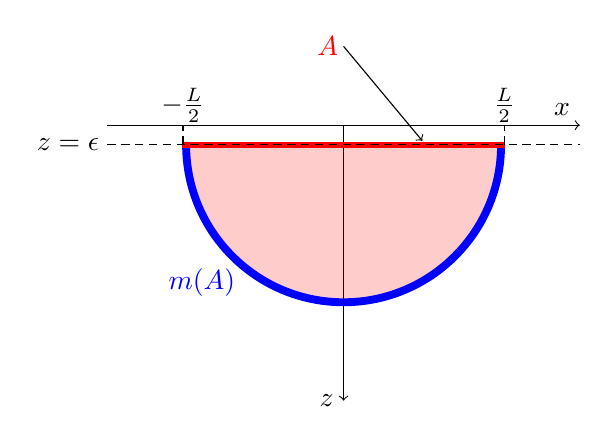
\begin{tikzpicture}[
        circ/.style={circle, draw, solid, fill=white, inner sep=0.75pt,
                     label=#1,
                     node contents={}
                     },
        every label/.append style = {inner sep=2pt, font=\footnotesize}
                            ]
        % shaded area
        
        % axis
        \draw[->]   (-6,0) -- + (6,0) node[above left] {$x$};
        \draw[->]   (-3,0) -- + (0,-3.5) node[left] {$z$};
        % rest of image
        \draw[fill=red,opacity=0.2] (-5,-.25) node[circ=below left:] arc (180:360:2) node[circ=below right:{}];
        \draw node at (-.96,.25){$\frac{L}{2}$};
        \draw node at (-5.04,.25){$-\frac{L}{2}$};
        \draw[blue, line width=1mm] (-5,-.25) arc (180:360:2);
        \draw[red, line width=.75mm] (-5.05,-0.25) -- (-.95,-0.25);
        %
        \draw[densely dashed]   (-5.04,-0.25) -- (-5.04,0);
        \draw[densely dashed]   (-.96,-0.25) -- (-.96,0);
        \draw[densely dashed]   (-6,-0.25) -- (0,-0.25);
        \draw node at (-6.5,-0.25){$z=\epsilon$};
        \draw[blue] node at (-4.8,-2.){$m(A)$};
        \draw[red] node at (-3.2,1){$A$};
        \draw[->]   (-3,1) -- + (1,-1.2);
    \end{tikzpicture}
    \caption{The blue curve represents the minimal bulk surface homologous to $A$ the red boundary slice. The dashed line is the z cutoff to prevent from UV divergences.}
    \label{Vacuum AdS}
\end{figure}

Consider a region $x\in\left[-L/2,+L/2\right]$ on the cutoff surface as presented in fig. \ref{Vacuum AdS},
\begin{align}
    x_0 = 0,        &&      r^2 = \left(\frac{L}{2}\right)^2+\epsilon^2.
\end{align}
Using (\ref{AdS_3 metric}) and (\ref{AdS_3 vaccum geodesic}), the length of the surface linking the two endpoints is easily computed and is found to be
\begin{equation}\label{first RT}
    m\left(A\right) = 2\ell\ln\left(\frac{L}{\epsilon}\right).
\end{equation}
Plugging this into the RT formula (\ref{RT}), and using the relation between the central charge and the AdS radius\footnote{In the limit of large number of field-theory degrees of freedom this relation is $c=\frac{3}{2G_\text{N}}\ell$.}, the entropy is
\begin{equation}
    S\left(A\right)= \frac{c}{3}\ln\left(\frac{L}{\epsilon}\right).
\end{equation}

The logarithmic divergence is expected from the term $\text{d}s\sim \ell \text{d}z/z$ in the metric.

\subsection{Holographic entanglement at finite temperature}

Now we derive the entanglement entropy of an interval on a circle $\Sigma$ of radius $R$, on which lives a CFT dual to a BTZ black hole in AdS$_3$.

Consider a holographic CFT on a circle $\Sigma$ of radius $R$. This system undergoes a \textbf{Hawking-Page} transition at temperature $T^*=\left(2\pi R\right)^{-1}$, \cite{Hawking1983}. This can be seen by comparing the free energies of the two possible geometries: thermal AdS and BTZ black hole. 
\begin{equation}
    \Delta F = F_{AdS}-F_{BTZ} = 2\pi^2\ell(LT^2-\frac{1}{L}),
\end{equation}
where $L=2\pi R$. Above this temperature, the bulk becomes a BTZ Black hole\cite{Ba_ados_1992},
\begin{align}\label{BTZ}
    \text{d}s^2 = \frac{\ell^2}{z^2}\left(-f\left(z\right)\text{d}t^2+\text{d}x^2+\frac{\text{d}z^2}{f\left(z\right)}\right),     &&      f\left(z\right)=1-\frac{z^2}{z_h^2}.
\end{align}
where $z_h$ is the position of the horizon and $x\sim x+2\pi R$. Using a Wick rotation $\tau=it$, we can show that $z_h$ is related to the Hawking temperature, see Appendix \ref{appendix B}.
\begin{equation}\label{Haking temperature}
    T = \frac{1}{2\pi z_h}.
\end{equation}

As the RT formula was introduced for pure states, it is not supposed to apply directly for the thermal state $\rho_\Sigma$. One should purify the state. One way to do this is through the thermofield double state, dual to the two-sided BTZ black hole, fig. \ref{Penrose diagram thermofield double}. But there are many other options to purify the thermal state as discussed in the previous chapter. This might be a problem if the minimal surface $m(A)$ depends on the choice of the purification. However, RT avoids this problem by a property called nesting. This property states that for any regions $A$ and $B$,
\begin{equation}
    r\left(A\right) \subseteq r\left(AB\right) = \sigma,
\end{equation}
where $r(A)$ is the the homology region of $A$. In this case the choice of purification is irrelevant. The nesting condition is but a geometric way to say that the state of a larger system determines the state of it subsystems.

However, there is one important equation that does not hold in the case of a thermal state,
\begin{equation}
    S\left(A\right)\neq S\left(A^c\right),
\end{equation}
which is what we should expect for a mixed state anyway.

\begin{figure}
     \centering
     \begin{subfigure}[b]{0.3\textwidth}
        \centering
        \begin{tikzpicture}
        \draw[name path = A] (1.82,-.829) arc (335.5:440.5:2);
        \draw[name path = AA] (1.82,-.829) arc (335.5:80:2);
            \begin{scope}
                \draw  [clip] (0,0) circle (2cm);
                \draw[color=red,line width=.6mm, name path = B] (1.82,-.829) .. controls (.51,.51) .. (0.32,1.974);
                \draw[color=blue,line width=.5mm, name path = R] (1.80,-.872) .. controls (.47,.47) .. (0.28,1.98);
                \tikzfillbetween[of=A and B]{red, opacity=0.2};
                \tikzfillbetween[of=AA and R]{blue, opacity=0.2};
            \end{scope}
            \draw[red] node at (2,1){$A$};
            \draw[blue] node at (-2,-1){$A^c$};
         \end{tikzpicture}
         \caption{}
         \label{fig_BTZ minimal surface a}
     \end{subfigure}
     \hfill
     \begin{subfigure}[b]{0.3\textwidth}
         \centering
         \begin{tikzpicture}
            \draw[name path = A] (1.82,-.829) arc (335.5:440.5:2);
            \draw[name path = AA] (1.82,-.829) arc (335.5:80:2);
            \draw[black,fill=black] (0,0) circle (.6cm);
            \begin{scope}
                \draw  [clip] (0,0) circle (2cm);
                \draw[color=red,line width=.6mm, name path = B] (1.82,-.829) .. controls (.51,.51) .. (0.32,1.974);
                \tikzfillbetween[of=A and B]{red, opacity=0.2};
                \tikzfillbetween[of=AA and B]{gray, opacity=0.2};
            \end{scope}
            \draw[red] node at (2,1){$A$};
         \end{tikzpicture}
         \caption{}
         \label{fig_BTZ minimal surface b}
     \end{subfigure}
     \hfill
     \begin{subfigure}[b]{0.3\textwidth}
         \centering
         \begin{tikzpicture}
            \draw[name path = A] (1.82,-.829) arc (335.5:440.5:2);
            \draw[name path = AA] (1.82,-.829) arc (335.5:80:2);
            \draw[red,fill=black,line width= .6mm] (0,0) circle (.6cm);
            \begin{scope}
                \draw  [clip] (0,0) circle (2cm);
                \draw[color=red,line width=.6mm, name path = B] (1.82,-.829) .. controls (-1.45,-.85) .. (0.32,1.974);
                \draw[color=blue,line width=.6mm, name path = R] (1.80,-.872) .. controls (-1.5,-.87) .. (0.28,1.98);
                \tikzfillbetween[of=A and B]{red, opacity=0.2};
                \tikzfillbetween[of=AA and R]{blue, opacity=0.2};
            \end{scope}
            \draw[red] node at (2,1){$A$};
            \draw[blue] node at (-2,-1){$A^c$};
         \end{tikzpicture}
         \caption{}
         \label{fig_BTZ minimal surface c}
     \end{subfigure}
     \hfill
    \caption{RT surfaces for a (a) pure state, and a (b,c) thermal state. In the case of a horizon in the bulk, there are many geodesics homologous to $A$. The choice between (b) and (c) is a result of minimizing the surface. This choice results in a sort of Page curve \ref{BTZ entropy phase transition}.}
    \label{fig_BTZ minimal surface}
\end{figure}

In the presence of a black hole, there are several possibilities regarding minimal surfaces as it can be seen in fig. \ref{fig_BTZ minimal surface}. As a matter of fact, there are an infinite number of geodesics indexed with their winding number around the black hole. Defining the region $A$ to be the boundary segment $\phi\in(0,L)$,  in the case $L\ll2\pi $, the obvious choice is that represented in fig. \ref{fig_BTZ minimal surface b}. It's length is
\begin{equation}\label{length BTZ red}
    2\ell\ln\frac{\sinh\left(\pi T L\right)}{\pi T\epsilon}.
\end{equation}
This result can be found by computing geodesics in a BTZ background as will be done in chapter \ref{section 6}.

In the case of large $L$, a second choice \ref{fig_BTZ minimal surface c} becomes possible as well. The geodesic winds (maybe multiple times) around the horizon. If we consider just the blue geodesic in fig. \ref{fig_BTZ minimal surface c}, $A$ does no longer satisfy the homology condition (we cannot continuously deform the geodesic to $A$), unless we add to it the horizon. In this case the minimal surface is,
\begin{equation}
    m\left(A\right) = m\left(A^c\right) + \mathcal{H}.
\end{equation}
It's length is 
\begin{equation}\label{length BTZ blue}
    2\ell\ln\frac{\sinh\left(\pi T \left(2\pi R-L\right)\right)}{\pi T\epsilon} + \left(2\pi\right)^2\ell RT.
\end{equation}

The entropy should be the minimum of the two equations (\ref{length BTZ red}) and (\ref{length BTZ blue}),
\begin{equation}\label{BTZ interval entropy}
    S\left(A\right) = \frac{c}{3}\min\left\{\ln\frac{\sinh\left(\pi T L\right)}{\pi T\epsilon}, 2\pi^2 RT + \ln\frac{\sinh\left(\pi T \left(2\pi R-L\right)\right)}{\pi T\epsilon}\right\}.
\end{equation}

This form of entropy will lead to a certain phase transition at a certain $L=L^*$ as plotted in fig. \ref{BTZ entropy phase transition}.

\begin{figure}
    \centering
    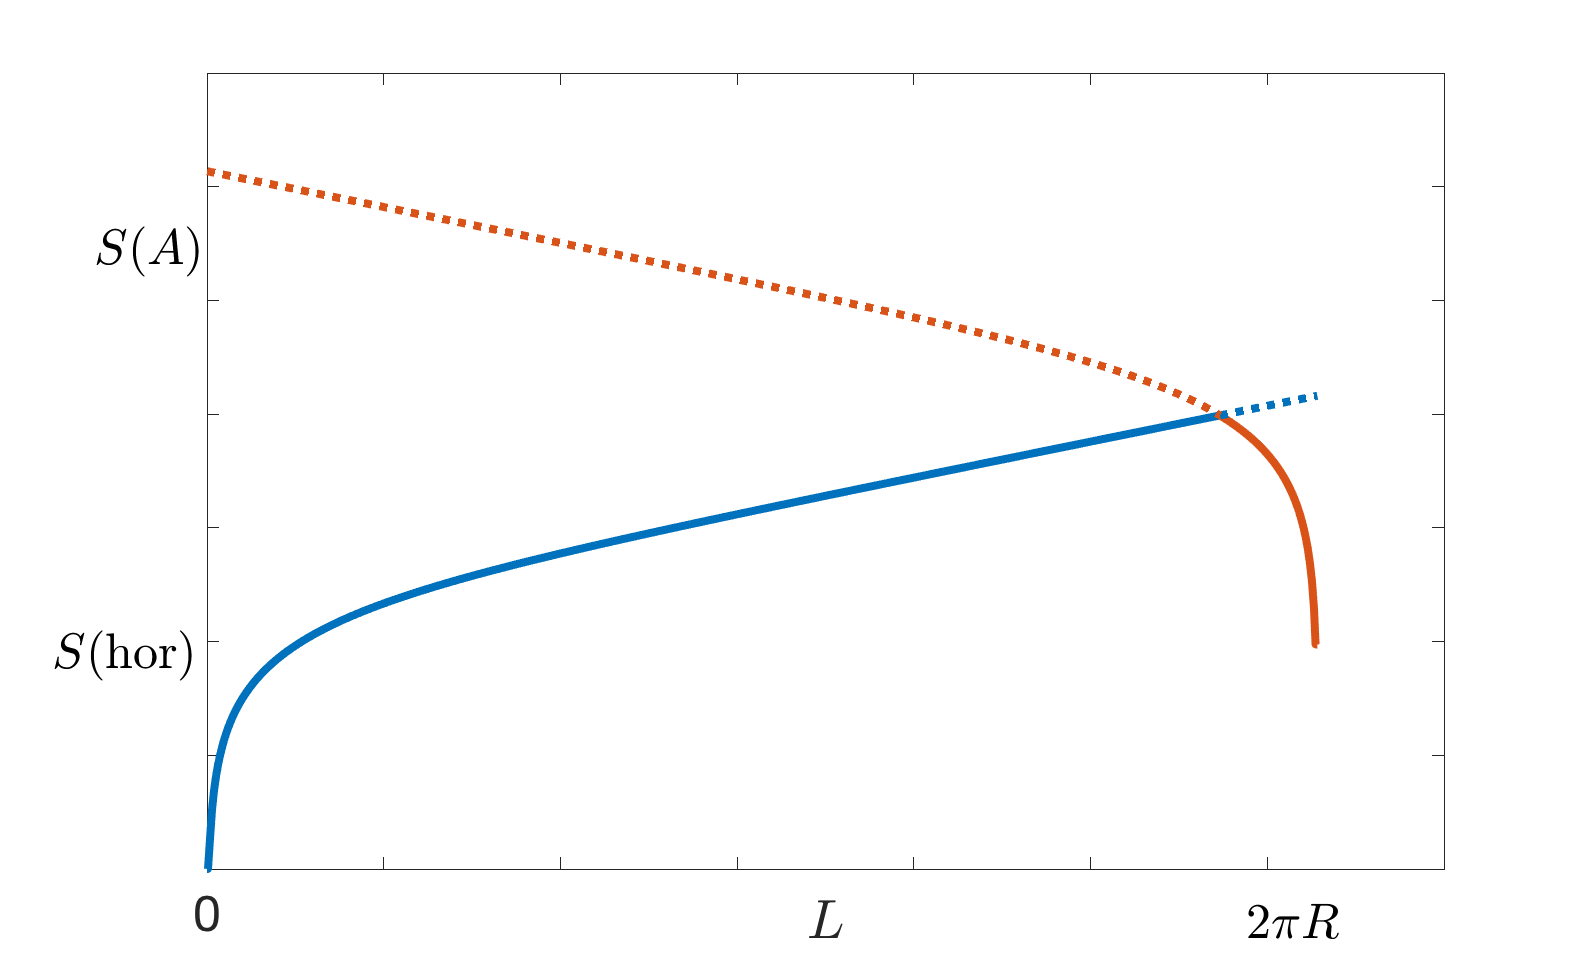
\includegraphics[width=0.65\textwidth]{figures/pagecurveplot0.png}
    \caption{The entropy of $A$ follows a sort of Page curve (\ref{BTZ interval entropy}). The minimal surface will switch from (\ref{length BTZ red}) to (\ref{length BTZ blue}) as $A$ becomes bigger. This resembles a phase transition.}
    \label{BTZ entropy phase transition}
\end{figure}
